\chapter{Προτεινόμενη Μεθοδολογία}
\label{chap4}

\section{Εισαγωγή}

Στις προηγούμενες παραγράφους είδαμε τη συνηθισμένη διαδικασία πρόβλεψης μιας χρονοσειράς:

\begin{enumerate}
\item Προετοιμάζουμε τα δεδομένα και τα φέρνουμε στην επιθυμητή μορφή για ανάλυση
\item Αποσυνθέτουμε τη χρονοσειρά στα επιμέρους συνθετικά της στοιχεία
\item Προεκτείνουμε με τις μεθόδου πρόβλεψης την αποεποχικοποιημένη χρονοσειρά στο μέλλον
\item Ενσωματώνουμε την εποχιακότητα στο μοντέλο πρόβλεψης
\item Αξιολογούμε την ακρίβεια της πρόβλεψης
\end{enumerate}

Μπορούμε όμως να παρατηρήσουμε ένα πρόβλημα στην παρακάτω διαδικασία. Στις περιπτώσεις που η χρονοσειρά μας δεν διαθέτει αρκετά ιστορικά δεδομένα, δεν είναι δυνατό για εμάς να εξάγουμε το στοιχείο της εποχιακότητας. Έτσι, διαχειριζόμαστε τη χρονοσειρά ως μη εποχιακή και εφαρμόζουμε τις μεθόδους πρόβλεψης στα αρχικά δεδομένα.  Είναι προφανές, όμως, ότι μπορούμε να έχουμε στη διάθεση μας χρονοσειρές που είναι εποχιακές και που θα μπορούσαμε να τις προβλέψουμε καλύτερα στη περίπτωση που είχαμε γνώση για την εποχιακή τους συμπεριφορά. 

Στη παρούσα διπλωματική προσπαθούμε να ξεπεράσουμε αυτό το πρόβλημα με χρήση της επιπλέον πληροφορίας που μπορούμε να λάβουμε από άλλες συναφείς χρονοσειρές με την υπό εξέταση χρονοσειρά. Έτσι, αν έχουμε στη διάθεσή μας δεδομένα που περιγράφουν παρόμοια μεγέθη, όπως λόγου χάρη πωλήσεις συναφών προϊόντων, υποθέτουμε ότι μπορούμε να εκμαιεύσουμε την ζητούμενη πληροφορία από το σύνολο των χρονοσειρών και να βελτιώσουμε την ακρίβεια της πρόβλεψης στις χρονοσειρές που στερούνται επαρκούς ιστορικού. 

\begin{figure}[t!]
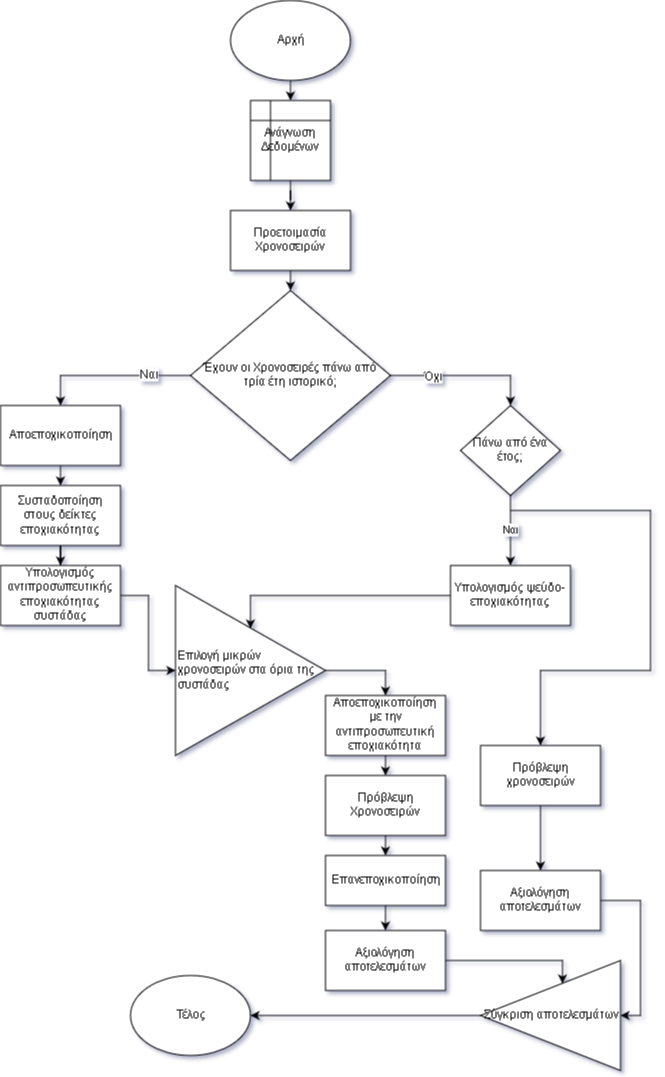
\includegraphics[scale=0.5]{figures/methodology.png}
\centering
\caption{Διάγραμμα Ροής Μεθοδολογίας}
\label{MethodologyFC}
\end{figure} 

Σε αυτό το κεφάλαιο θα περιγράψουμε πώς εξετάστηκε αυτή η υπόθεση. Αρχικά, φέρνουμε τα δεδομένα μας σε κατάλληλη μορφή για την στατιστικές μεθόδους που θέλουμε να εφαρμόσουμε. Έπειτα, χωρίζουμε τις χρονοσειρές σε δύο ομάδες: εκείνες με επαρκές ιστορικό για να εξάγουμε το στοιχείο της εποχιακότητας και τις υπόλοιπες. Στη πρώτη κατηγορία, εντοπίζουμε τους δείκτες εποχιακότητας κάθε χρονοσειρά και κατόπιν εξετάζουμε αν υπάρχει συνάφεια μεταξύ τους. Το αποτέλεσμα είναι να δημιουργηθούν συστάδες με παρόμοια εποχιακότητα και υπολογίζουμε τους αντιπροσωπευτικούς δείκτες εποχιακότητας της συστάδας. Στις χρονοσειρές που στερούνται επαρκής πληροφορίας, προσπαθούμε να βρούμε μία ψεύδο-εποχιακότητα που θα χρησιμοποιήσουμε σαν κριτήριο συνάφειας με τις συστάδες που προέκυψαν προηγουμένως. Για τις μικρές χρονοσειρές που βρέθηκε να παρουσιάζουν παρόμοια εποχιακή συμπεριφορά με κάποια ομάδα, εφαρμόζουμε τα μοντέλα πρόβλεψης κάνοντας αποεποχικοποίηση με του λόγους εποχιακότητας της συστάδας. Κατόπιν κάνουμε πρόβλεψη στις ίδιες χρονοσειρές χωρίς αποεποχικοποίηση. Τελικώς, συγκρίνουμε τα αποτελέσματα των δύο προσεγγίσεων. 

Μια αναπαράσταση της διαδικασία μπορούμε να δούμε στο διάγραμμα ροής του σχήματος \ref{MethodologyFC}.

\section{Προετοιμασία και Αποσύνθεση Χρονοσειρών}

\subsubsection{Έλεγχος τιμών, \en{resampling} και διαχείριση κενών τιμών}
Αρχικά, πρέπει να φέρουμε τα δεδομένα σε μία μορφή κατάλληλη για την ανάλυση και εφαρμογή μεθόδων που θέλουμε να κάνουμε. Για να το πετύχουμε αυτό εφαρμόζουμε τις τεχνικές επαναδειγματοληψίας και διαχείρισης κενών τιμών που αναπτύξαμε στο προηγούμενο κεφάλαιο, αφότου έχουμε επιλέξει από το σύνολο δεδομένων μας τη πληροφορία που μας είναι χρήσιμη. 

Βέβαια, η παραπάνω διαδικασία δεν μπορεί να γίνει μόνο ως κλειστό κουτί (\en{black box}, δηλαδή να διαχειρίζεται πλήρως από το σύστημά μας. Πρέπει να αποκτήσουμε μία εποπτική διαίσθηση πάνω στα δεδομένα και στηριζόμενοι στη γνώση που έχουμε για τη φύση τους να διορθώσουμε τυχούσες ατέλειες. Μία συχνή τέτοια περίπτωση είναι οι αρνητικές τιμές σε ένα φυσικό μέγεθος που δεν δύναται να παίρνει τέτοιες. 

Με παρόμοιο τρόπο πρέπει να σχεδιάσουμε τη διαδικασία του \en{resampling} και της διαχείρισης κενών τιμών. Ο λόγος είναι ότι καλούμαστε να επιλέξουμε τη κατάλληλη συνάρτηση ή προσέγγιση για να γίνουν τα παραπάνω και για να μην αλλοιωθεί η πληροφορία που φέρουν τα δεδομένα κατά αυτή τη διαδικασία, πρέπει να ορίσουμε ένα σύνολο φυσικών κανόνων που απορρέει από το προσδιορισμό της φύσης τους.

Τελικά, για να μπορέσουμε να αξιολογήσουμε τη προτεινόμενη μέθοδο πρέπει να αποκρύψουμε τις τελευταίες τιμές των χρονοσειρών μας. Το χρονικό διάστημα που αφαιρούμε από τα δεδομένα θα αποτελέσει και τον ορίζοντα πρόβλεψης των μοντέλων που θα χρησιμοποιήσουμε. Έτσι, το αποτέλεσμα των μεθόδων θα συγκριθεί με τις κρυμμένες τιμές και θα έχουμε τη δυνατότητα να αξιολογήσουμε την ακρίβεια της προσέγγισής μας.

\subsection{Αποεποχικοποίηση}

Οι μέθοδοι αποεποχικοποίησης που συναντήσαμε στο Κεφάλαιο 2, απαιτούν η αρχική μας χρονοσειρά να έχει επαρκές πλήθος δεδομένων. Κάνουμε μια διαμέριση, λοιπόν, των δεδομένων μας σε δύο ομάδες: αυτές που έχουν πάνω από τρία έτη παρατηρήσεων και αυτές που δεν έχουν. 

Ικανοποιούνται τα κριτήρια για την αποσύνθεση στη πρώτη ομάδα χρονοσειρών και εφαρμόζουμε το πολλαπλασιαστικό μοντέλο της κλασσικής μεθόδου αποσύνθεσης. Το γεγονός ότι σκοπεύουμε να χρησιμοποιούμε τους δείκτες εποχιακότητας που θα προκύψουν ως το σημείο αναφοράς για να εντοπίσουμε τις συστάδες που υπάρχουν στο σύνολο των δεδομένων μας, καθιστά την διασφάλιση της υψηλής ακρίβειας ακόμα πιο σημαντική κατά τον υπολογισμό τους. Έτσι, χρησιμοποιούμε τη μέθοδο συρρίκνωσης \en{James-Stein} κατά τη διαδικασία υπολογισμού των λόγων εποχιακότητας. Επίσης, είναι απαραίτητο όλες οι χρονοσειρές να έχουν τους δείκτες τους στην ίδια κλίμακα και συνεπώς κανονικοποιούνται έτσι ώστε το άθροισμά τους να είναι ίδιο με το μήκος της εποχιακότητας.

Πρέπει, όμως, να μπορέσουμε να αποκτήσουμε και μια εικόνα για την εποχιακότητα των χρονοσειρών που στερούνται επαρκές πλήθος παρατηρήσεων. Έτσι, για τις υπόλοιπες χρονοσειρές, θα χρησιμοποιήσουμε τους εξής τύπους για να λάβουμε το σύνολο των ``ψεύδο-εποχιακών'' δεικτών:

\[ CxSxR = \frac{Y}{LRL} \]

Θέτουμε την τάση της χρονοσειράς να είναι ίση με την ευθεία γραμμικής παλινδρόμησης επί των δεδομένων. Θεωρώντας ότι η χρονοσειρά μας είναι πολλαπλασιαστική, αφαιρούμε την τάση από τα αρχικά δεδομένα διαιρώντας την αρχική χρονοσειρά με την ευθεία ελαχίστων τετραγώνων.

\[ PS_t = mean(CxSxR_t, CxSxR+{t+l_{season}}, \dots, CxSxR_{t+i*l_{season}}), \]
\[ t+i*l_{season} < L, i=1,2,\dots \] 
\[ PS_{norm} = \frac{ PS * l_{season}}{\sum{PS_t}} \]

Όπου, PS είναι η σειρά της ψευδο-εποχιακότητας, $l_{season}$ το μήκος της εποχιακότητας και $L$ το μήκος της χρονοσειράς. Συνεπώς, ορίζουμε την ψευδο-εποχιακότητα ως το μέσο όρων των τιμών ανά περίοδο της χρονοσειράς, αφότου της έχουμε αφαιρέσει την τάση. Κατόπιν, κανονικοποιούμε το προηγούμενο αποτέλεσμα έτσι ώστε το άθροισμα των δεικτών ψευδο-εποχιακότητας να αθροίζει στο μήκος του εποχιακού μοτίβου. 

\section{Συσταδοποίηση Δεικτών Εποχιακότητας}

Έχοντας το σύνολο των εποχιακών δεικτών μπορούμε πλέον να εφαρμόσουμε ανάλυση συστάδων \en{(cluster analysis)} σε αυτό. Μας ενδιαφέρει το σύνολο των χρονοσειρών των οποίων η εποχιακότητα προέκυψε με τις κλασικές μεθόδους αποσύνθεσης. 

Για να το καταφέρουμε αυτό, θα χρησιμοποιήσουμε μεθόδους συσταδοποίησης (\en{clustering}) από το πεδίο της Μηχανικής Μάθησης (\en{Machine Learning}). Δύο μέθοδοι που ελέγξαμε είναι οι μέθοδοι \en{k-means} και \en{DBSCAN}. 

\subsection{\en{K-means}}

Ο αλγόριθμος \en{K-means} γνωστός και ως ο αλγόριθμος του \en{Lloyd}, παράγει οικογένειες δεδομένων που χαρακτηρίζονται από παρόμοια διακύμανση, προσπαθώντας να ελαχιστοποιήσει την ενδοοικογενειακό τετραγωνική διαφορά. Το πλήθος των συστάδων που θα προκύψουν από την εφαρμογή του αλγορίθμου είναι μία παράμετρος που ορίζει ο χρήστης.

Κάθε συστάδα (\en{cluster}) χαρακτηρίζεται από το κέντρο της (\en{centroid}), που ουσιαστικά είναι ο μέσος όρος όλων των στοιχείων που την αποτελούν. Βάσει αυτού, υπολογίζεται το κριτήριο της τετραγωνικής διαφοράς μια συστάδας, που προσπαθεί ο αλγόριθμος να ελαχιστοποιήσει.

Η μέθοδος χαρακτηρίζεται από τρία βασικά βήματα, που μετά το πρώτο ο αλγόριθμος επαναλαμβάνει τα άλλα δύο:

\begin{enumerate}
    \item Επιλογή αρχικών κεντρών για τις συστάδες
    \item Κατανομή των στοιχείων (εδώ χρονοσειρών) σε συστάδες, ανάλογα με την απόσταση από το κέντρο τους
    \item Υπολογισμός νέου κέντρου κάθε συστάδας, ως ο μέσος όρος των στοιχείων που την αποτελούν
\end{enumerate}

Ο αλγόριθμος σταματάει, όταν δεν έχουμε μεγάλη διαφορά μεταξύ των κεντρών που υπολογίστηκαν ανάμεσα από δύο επαναλήψεις. 

\subsection{\en{DBSCAN}}

Ο αλγόριθμος \en{DBSCAN (Density-Based Spatial Clustering of Applications with Noise)} αντιμετωπίζει τις συστάδες ως περιοχές που χαρακτηρίζονται από μεγάλη πυκνότητα και χωρίζονται μεταξύ τους από περιοχές που δεν έχουν αυτό το χαρακτηριστικό. Έτσι, σε αντίθεση με τον \en{K-means} μπορεί να παράξει συστάδες που δεν χρειάζεται να είναι σε κυρτές περιοχές του χώρου.

Στον αλγόριθμο \en{DBSCAN} δεν χρειάζεται να οριστεί από πριν το πλήθος των συστάδων, ενώ αντιμετωπίζει κάποια στοιχεία του συνόλου ως ακραίες τιμές που δεν κατατάσσει σε καμία συστάδα. Όμως, πρέπει να οριστεί τι εννοούμε πυκνή περιοχή και αυτό γίνεται με δύο παραμέτρους. Ένα βασικό στοιχείο της μεθόδου είναι τα βασικά δείγματα \en{core samples}, δηλαδή ένα δείγμα από το σύνολο των δεδομένων μας που έχει τουλάχιστον \textit{ν} το πλήθος άλλα στοιχεία του συνόλου, το πολύ σε απόσταση \textit{ε} από αυτό. Τα \textit{ν} και \textit{ε} είναι οι παράμετροι που ορίζουν πόσο πυκνό πρέπει να είναι ένα \en{cluster}.

\subsection{Επιλογή και εφαρμογή μεθόδου}

Ζητούμενο σε αυτό το βήμα της μεθοδολογίας είναι να ελέγξουμε αν πράγματι υπάρχει συνάφεια στην εποχιακή συμπεριφορά των χρονοσειρών που έχουμε στη διάθεσή μας και να κάνουμε συστάδες βάσει αυτού. Συνεπώς, η ανάλυση συστάδων γίνεται με χρήση του αλγορίθμου \en{DBSCAN}. 

Εντοπίζουμε με πειραματισμό τις κατάλληλες παραμέτρους για τον αλγόριθμο. Κριτήριο μας είναι τα \en{cluster} που προκύπτουν να μην έχουν μικρό αριθμό, έτσι ώστε να μπορεί να παραχθεί αντιπροσωπευτική εποχιακότητα μέσα από αυτό.

Έχοντας παράξει τα \en{clusters} με εφαρμογή του αλγορίθμου, πρέπει να δούμε αν οι υπόλοιπες χρονοσειρές βάσει των ψευδο-εποχιακών δεικτών, θα μπορούσαν να ανήκουν σε αυτά. Ένας τρόπος για να το διαπιστώσουμε αυτό είναι να το ελέγξουμε βάσει του κριτηρίου των τετραγώνων του \en{K-means}. Έτσι, ελέγχουμε ποια είναι η μέγιστη τετραγωνική απόσταση μέσα σε κάθε συστάδα από το κέντρο της. Αν η απόσταση της ψευδο-εποχιακότητας μιας χρονοσειράς έχει μικρότερη απόσταση από το κέντρο της συστάδας από αυτή που υπολογίσαμε, τότε την κατατάσσουμε σε αυτή. 

Τελικώς προκύπτει ένα υποσύνολο των χρονοσειρών που δεν είχαν αρκετές παρατηρήσεις να προσεγγίζουν την εποχιακή συμπεριφορά άλλων που είχαν. Έτσι μπορούμε να περιμένουμε ότι πράγματι είναι εποχιακές χρονοσειρές και χρησιμοποιώντας το κέντρο της συστάδας που την κατατάξαμε, να την αποεποχικοποιήσουμε. Μένει να δούμε αν προβλέποντας κατά αυτό τον τρόπο αποεποχικοποιημένη χρονοσειρά μπορούμε να έχουμε καλύτερα αποτελέσματα από το να κρίναμε αυτές τις χρονοσειρές μη εποχιακές και να τις προεκτείναμε ως τέτοιες.

\section{Πρόβλεψη}

Για την πρόβλεψη, τόσο των αποεποχικοποιημένων χρονοσειρών όσο και των αρχικών τους δεδομένων θα χρησιμοποιήσουμε τις μεθόδους που είδαμε στο Υποκεφάλαιο 3.3. Συγκεκριμένα θα χρησιμοποιήσουμε τις εξής μεθόδους:

\begin{itemize}
  \item \en{Naive}
  \item Γραμμική Παλινδρόμηση (\en{LRL})
  \item Απλή Εκθετική Εξομάλυνση (\en{SES})
  \item Εκθετική Εξομάλυνση Γραμμικής Τάσης (\en{Holt Exponential Smoothing})
  \item Εκθετική Εξομάλυνση Φθίνουσας Τάσης (\en{Damped Exponential Smoothing})
  \item Κλασική Μέθοδο Θ (\en{Theta Classic})
\end{itemize}

Για να βρεθούν οι βέλτιστες τιμές των παραμέτρων για κάθε μία από τις μεθόδου που εφαρμόζουμε εδώ, χρησιμοποιήθηκε το μέσο τετραγωνικό σφάλμα \en{MSE}. Συγκεκριμένα, ελέχθησαν όλες οι δυνατές τιμές των παραμέτρων με βήμα 0.01 και εκείνες που παρήγαγαν το μικρότερο μέσο τετραγωνικό εντός-του-δείγματος σφάλμα (\en{out-of-sample error}) χρησιμοποιήθηκαν για την επέκταση της χρονοσειράς στο μέλλον. 

Οι παραπάνω μέθοδοι εφαρμόστηκαν δύο φορές. Μία αφότου αποεποχικοποιήσαμε τα δεδομένα και μία στην αρχική τους μορφή. Στη πρώτη περίπτωση ενσωματώθηκε στο μοντέλο της πρόβλεψης και η εποχιακότητα της συστάδας στην οποία άνηκε η εκάστοτε χρονοσειρά.

\section{Αξιολόγηση Πρόβλεψης}

Το σημαντικότερο βήμα της διαδικασίας, καθότι αξιολογώντας της κάθε προσέγγιση και συγκρίνοντας τα αποτελέσματα μπορούμε να αποφανθούμε αν πράγματι η λύση του προβλήματος για τις μικρές εποχιακές χρονοσειρές, που προτείνεται στη παρούσα διπλωματική, προσφέρει βελτίωση στην ακρίβεια.

Στο πρόβλημα αυτό εφαρμόζουμε τον δείκτη ακριβείας σε ένα μεγάλο πλήθος χρονοσειρών που μπορεί να χαρακτηρίζεται από διαφορετικά επίπεδα στις χρονοσειρές που εμπεριέχει. Γι' αυτό τον λόγο χρειαζόμαστε ένα σφάλμα που είναι στην ίδια κλίμακα για όλες τις χρονοσειρές και παράγει διαφορετικά αποτελέσματα ανάλογα με το μέγεθος των παρατηρήσεων.

Επίσης, η χρονοσειρές, λόγω και της εποχιακότητας που τις χαρακτηρίζει, θα έχουν τιμές σε κάποιες χρονικές περιόδους που είναι πιθανό να βρίσκονται πολύ κοντά στο μηδέν. Ο δείκτης που θα χρησιμοποιήσουμε, λοιπόν, δε πρέπει να είναι ευαίσθητος στις μικρές τιμές.

Ένας δείκτης που μπορούμε να ορίσουμε που ικανοποιεί τα προαναφερθέντα κριτήρια είναι ο κανονικοποιημένος δείκτης μέσο απόλυτου σφάλματος που δίνεται από τον ακόλουθο τύπο:

\[ MAE_{norm} = mean(e_i)/mean(Y) \]

Βάσει, λοιπόν, αυτού του δείκτη βλέπουμε αν η μέθοδος μας παράγει καλύτερα αποτελέσματα ανά μέθοδο. Αυτό μπορούμε να το δούμε τόσο στο κατά μέσο όρο σφάλμα ανά μέθοδο όσο και στο ποσοστό των χρονοσειρών που παρουσίασαν πιο ακριβείς προβλέψεις με τη προτεινόμενη προσέγγιση. 

Χρησιμοποιώντας τη πληροφορία που λάβαμε από το τελευταίο βήμα, μπορούμε να δούμε πώς θα μπορούσαμε να βελτιώσουμε τη μεθοδολογία εν συνόλω.


